%Obviously, here you describe in great detail the actual analysis you conducted. The level of detail should be sufficient to allow a very smart fellow student in your field to reproduce more or less your research.
%Therefore, in MOTDOP, there may be multiple optimal solutions with different trade-offs among the scores, which are called the Pareto optimal solutions. In multi-objective optimization, solution a is said to dominate solution b, if all the objective values of a are no worse than that of b, and there is at least one objective for which a has a better value than b. Then, a solution is called to be a Pareto optimal solution, if it is dominated by no other solution in the entire solution space.
%euclidean distance between a and b

\chapter{Solution Development}\label{chapter:analysis}
In a previous work on this topic, Wörndl \& Herzog  \parencite{cbrecsys2014} drew inspiration for their formal model from the Oregon Trail Knapsack (see \ref{sec:oregon}). They formulated a model that extends the value function of the Oregon Trail Knapsack problem by a penalty function.

For clarity, we shall adjust the notation used in their paper to fit the notations used in previous function values. They formally defined their value function as:

\begin{gather}
 \tag{1} f_j(x_j, x_{d_j}) = x_j \cdot v_j - \sum_{e \in x_{d_j}} ( t(j, e) \cdot x_j \cdot v_j \cdot [x_e > 0])\label{eq:3d}
\end{gather}

where $v_j$ is the value of region $j$ (i.e, item) for the specified user query and $t(j, e)$ is the penalty function for two regions $j$ and $e$. Their value function is similar to the function \ref{eq:2g} specified by the original Oregon Trail Knapsack model. However, the previously defined value reducing constant factor $t$, was a function of the two regions $j$ and $e$. 

Their formal model was defined as follows:
\begin{align}
    \tag{1}maximize \qquad  &\sum_{i=1}^n  f_j(x_j, x_{d_j}) \label{eq:3a}\\
    \tag{2}subject \ to \qquad &\sum_{i=1}^n x_i d_i  \leq D \label{eq:3b}\\
    \tag{3}&\sum_{i=1}^n x_i\ b_i \leq B \label{eq:3c}\\
    \tag{4} &x_i \in \{0,1\}
\end{align}

where $f_j(x_j, x_{d_j})$ is the penalty function defined in \ref{eq:3d}. $d_i$ is item i's recommended duration of stay and $b_i$ is item i's recommended daily budget. $D$ is the maximum possible duration of stay and $B$ is the maximum budget the user can spend on her trip. 

Already, Wörndl \& Herzog had concluded that the penalty function defined in their work could be improved to ensure better results. Penalty-based function require careful considerations of the function parameters and the function itself. Thus, to gain freedom from the influence of the penalty function, we shall be reformulating and extending the problem definition to a non-penalty based approach. It is to note that, if from further analysis, a penalty-based approach proves to be a better fit for our selected algorithm, then we shall redefine a penalty function as needed. 

The framework for our recommender system comprises a knapsack model for the multi-objective orienteering problem, a data model, and a meta-heuristic solution. In this section, we shall be analyzing these three parts in great detail. 


\section{Problem Reformulation} \label{sec:problem_definition}

Let us consider $n$ regions, $(i = 1, ..., n)$. Each region $i$ will have $k$ profits $s_{ik}\ (p = 1, ...,k)$. Given a set $N$ of $m$ traveling preferences $N = \{N_1, N_2,...,N_m\}$, $s_{ik}$ is dependent on $i$'s score on $N$. For example, a region can have a different score for shopping and another for hiking.
The recommendation problem can be modeled as a multi-objective orienteering problem. Given a user query, some regions must be selected to maximize the $p$ total profits while not exceeding a budget limit $B$ and a total stay duration $D$. Each user preference must be fulfilled by at least one of the selected regions. Assuming the system recommends a trip $T$ which comprises $n$ regions ($T = {x_1, x_2, ..., x_n}$, the physical distance between a region $x_i$ and its neighbor $x_2$ should not exceed a defined constant $\sigma$. In the case where no location coordinates on the regions are possible, the regions in the recommended trip should be within reasonable distance from each other. Also, the duration of stay in a particular region ${x_i}$ should ensure a minimum utility value. The utility value is to be defined in the algorithm.

The mathematical model of the \gls{moop} can be defined as follows:

\begin{align}
    \tag{1}maximize \qquad  &z_n(x) = \sum_{k=1}^p x_i\ s_{ik}, \hspace{1cm} i = 1,...,n \label{eq:3_1a}\\
    \tag{2}subject \ to \qquad &\sum_{i=1}^n x_i\ d_i  \leq D \label{eq:3_1b}\\
    \tag{3}&\sum_{i=1}^n x_i\ b_i \leq B \label{eq:3_1c}\\
    \tag{4}&\sum_{j \in N} x_{ij} \geq 1 \label{eq:3_1e}\\ 
    \tag{5}&\sum_{i=1}^n x_{i} \ g(p_i) \leq \sigma,  \hspace{1cm}  \label{eq:3_1f} \\
    \tag{7} x_i \in \{0,1\}, \qquad &\forall \ 1 \leq i \leq n
\end{align}
where $x_i = 1$ when an item $i$ is chosen, else $x_i = 0$. 
The constraint \ref{eq:3_1b} and \ref{eq:3_1c} represent the constraint on the total stay duration and the budget, respectively. Equation \ref{eq:3_1e} ensures that each user preference is satisfied at least once. The constraint \ref{eq:3_1f} denotes the constraint on the physical distance between the regions, whereby $g$ is a function of the physical location of the item. It is assumed that all coefficients $s_{ik}, b_{i}, B, d_i,$ and $D$ are positive. 

\subsection{Pareto Optimum}
There are multiple scores to be maximized in the objective function. Therefore, choosing an objective maximizing optimal solution without trade-offs is near infeasible. In multi-objective optimization, a solution $s$ is said to dominate $s'$ if $s$ is at least as good as $s'$ on every criterion, and $s$ is better in at least one criterion. $s \succ s'$ is used to write such case. If no solution dominates the solution $s^*$, then $s^*$ is said to be \textit{Pareto optimal} (i.e., non-dominated). The set of all non-dominated vectors is known as the \textit{Pareto front}.

\textbf{Example}:
Figure \ref{fig:moopsample} illustrates a bi-objective sample instance of the \gls{moop} problem. For simplicity, we assume two given preferences. The gray box display the user input. When mapped to our problem definition, there are two objectives to be maximized, where an objective represents a single item. An item can be any \gls{poi} (for example, attraction sites, region, or route). $f = (\Vec{f_1}, \Vec{f_2}, ... ,\Vec{f_k})$ represents all feasible solutions. We compute a solution in the objective space $\Vec{f_i} = (z_1, z_2)$. The objective values are computed on preferences $M$ \& $S$, while respecting the necessary constraints. The parameter $x$ in the illustration is a boolean array to encode the selection of an item combination. The selected item combinations are subject to the notion of Pareto optimality we have defined earlier. For example, $f_7 \succ f_2$ because it is at least as better in one of its objective value as $f_2$ and it is strictly better in another value. The Pareto front consists of the selections $\{f_1,f_5,f_7,f_9,f_{10}\}$, and we achieve a total score of (24, 23). 


\begin{figure}[ht!]
    \centering
    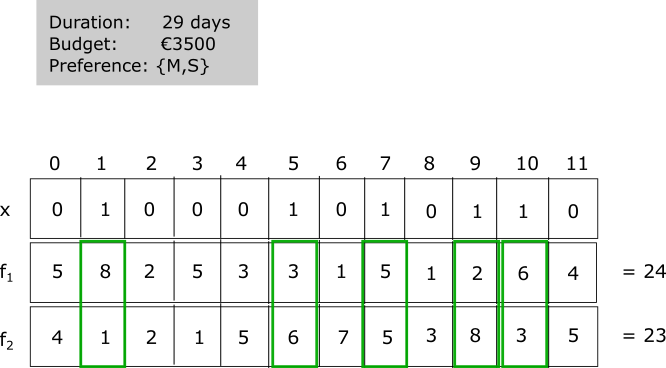
\includegraphics[width=8cm]{Moop}
    \caption{Example solution to the multi-objective orienteering problem}
    \label{fig:moopsample}
\end{figure}

Pareto's optimality here implies that there is no item combination $f_k$ that will improve the score achievable in one item without diminishing the achievable score in at least another item. 

We can also extend the concept of Pareto optimality from the solution space to the objective space. Given $n$ objective functions $z = (z_1,...,z_n)$, with each objective having a score $\Vec{v} = (v_1,...,v_j)$ on $j$ criteria, we define the concept of Pareto optimality in the objective space as follows. An objective $z$ dominates an objective $z'$, denoted by $z \succ z'$, if
\begin{itemize}
    \item $z_i(v) \geq z_i'(v)$ on each score of $\Vec{v_j}$; and
    \item there exists one score $v^*$ such that $z_i'(v^*) > z_i'(v)$.
\end{itemize}

Again, Pareto optimality here implies that there is no feasible objective $z_i$ that $v'$ without making it worse off in at least one other criterion. \newline Having gained a better understanding of what is deemed optimal, an algorithm that can efficiently compute the Pareto front from a set of given items is what we aim to develop in subsequent sections.


\section{Data Model}
%Describe in detail which data you use and how you collect these data. This may include qualitative data ("I analyze these in-depth travel behavior surveys."), or statistics you use, or data you collect yourself. The description should be as detailed that a very good fellow student in your field would be able to more or less reproduce your work. If you conduct a case study, the study area needs to be introduced here.
\note{Current thinking: child regions with same parents are within the same proximity}
\todo{Research traveller type and categorize preferences under classes for the multiple choice knapsack classes}

\section{Analysis of Algorithmic Methodologies}\label{sec:alg_approaches}
According to Golden et al. \parencite{Golden1987TheProblem}, \gls{op} is an NP-Hard problem. Hence, no known or expected algorithm can solve the problem optimally in polynomial time (i.e., an exact solution cannot be found within a reasonable amount of time). Computing an optimal solution with multiple objectives is even more intractable. Hence, there is usually a trade-off between time and accuracy. In multi-objective optimization, one is often interested in the Pareto front. However, it is usually infeasible to generate the exact set of Pareto front. A reason could be that the number of Pareto optima is too large, or the determination of a single Pareto optimum is computationally hard. Therefore, the goal is usually to identify a satisfactory Pareto set approximation (i.e., a set as close to the optimum as possible \parencite{Fonseca2005AOptimizers}. Approximate algorithms offer near-optimal solutions to computationally intractable problems (mostly) in a moderate amount of time and are the major alternative to solving NP-Hard class of optimization problems.

Approximate algorithms can be classified as heuristics and meta-heuristics. Heuristics are usually problem-dependent and inflexible (i.e., defined for a specific problem). Meta-heuristics are problem-independent and can be applied to a broad range of optimization problems. In section \ref{chapter:literature_review}, we discovered that meta-heuristic solutions were commonly used to solve \glspl{op}. Meta-heuristic solutions are also commonly used in multi-objective optimization for different research areas. 
Certain requirements must be considered when designing or selecting an appropriate algorithm to solve the \gls{moop}. Some requirements are intuitive for our problem domain. For example, a slow computational time by the end algorithm is intolerable for a user-oriented system. Some are not so intuitive. Uniform diversity preserving implies that the selected solutions in the approximated Pareto front are diverse and uniformly distributed. Also, the \gls{moop} has been defined such that a single objective represents a single user's preference. We are unable to pre-determine the number of preferences a user might select. A user could have just one preference. They might also have two or more preferences. Therefore, an appropriate algorithm should be applicable to a dynamic amount of objectives. A brief summary of the most important requirements of the desired algorithm is as follows.
\begin{itemize}
    \item Tolerable computational time
    \item Applicability to problem domain
    \item Uniform diversity Preserving
    \item Applicability to large-sized problem
    \item Applicability to dynamic amount of objectives
    \item Moderate implementation Complexity
\end{itemize}



To develop an algorithm to solve our optimization problem, first, we will discuss the basic methodologies in designing an approximation algorithm. Then we shall analyze possible heuristic and meta-heuristics solutions. All through this section, we assume a maximization problem where function $g$ means $f_k$ has to be maximized.   

\subsection{Greedy Methods}
Greedy methods help find suboptimal solutions that satisfy some performance guarantee in NP-Hard problems. The idea is to generate a solution incrementally by making the best possible choice according to a simple criterion at each decision-making point. For example, a greedy approach to solving the simple knapsack problem is to select a node with the least amount of weight iteratively. They are best used together with some form of heuristic rather than a stand-alone method. When used alone, they generate only a minimal number of different solutions.


\subsection{Local Search}
Local search techniques range from simple heuristics to complex meta-heuristics. The basic idea behind local search is to start from an initial (partial or non-partial) \gls{candidate solution}. The solution is improved by making local changes to it and moving from one \gls{candidate solution} to a neighboring \gls{candidate solution} until no further improvement is possible. A local change might involve removing elements from the ground set, adding elements, or swapping elements. Local search is a good heuristic for computing near-optimum solutions to reasonably sized problems. Usually, a neighborhood function $N: S \mapsto 2^S$ where $S $ is the set of feasible solutions, specifies for each solution $s \in S$ a subset $N(s)$ of neighbors of $s$ (neighborhood relation), or solutions that are close to $s$ \parencite{Gonzalez2007HandbookMetaheuristics}.

For many problems, computing the locality gap (i.e., the difference between local and global optima) is complex, and the locality gap using local natural search is commonly very large. Also, the algorithm might visit the exact location within the search space more than once. Thus, it can get trapped in a location far away from the global optimum. These all lead to very poor approximation. Consequently, many local search techniques use mechanisms to help escape a position or reduce the locality gap. For example, one could use a restart strategy when stuck in a local minimum in the iterative descent algorithm. Alternatively, one could relax the improvement criterion by performing a non-improving step. However, these strategies do not guaranty escaping an arbitrary local minimum \parencite{HolgerH2005StochasticSearch}.


\subsubsection{Iterative Improvement}
The iterative improvement algorithm is the most basic local search algorithm and forms the basis of the idea of most local search algorithms. Algorithm \ref{alg:iterative-improvement} (\textit{IterativeDescent)} shows a simple iterative improvement (also known as iterative descent). The solution of the iterative descent is the optimum local value, which may or may not be a global optimum. Condition $g(s') > g(s)$ is known as the evaluation of the candidate solution. Evaluation functions serve as guidance to a solution \parencite{HolgerH2005StochasticSearch}. In optimization problems, the objective function's properties usually determine the evaluation function. Below, the algorithm assumes a maximization objective function. 

 \begin{algorithm}
  \caption{General Outline of Iterative Improvement Local Search}\label{alg:iterative-improvement}
  \SetKwInOut{Input}{Input}
  \SetKwInOut{Output}{Output}
  \Input{Set of candidate solutions $S$, Neighborhood function $N$, Objective function $g$}
  \Output{A local optimum solution $s \in S$}
    determine an initial candidate solution $s$
    
    \While {$N(s)$ contains better solution than $s$}{
        choose a solution $s' \in N(s)$ such that\\
             \hspace{0.5cm}$g(s') > g(s)$\\
        $s := s'$\\
    }
  \end{algorithm}
  
The simple iterative improvement algorithm can be extended to multi-objective optimization problems. For multiple objectives, the solution of the iterative improvement and all local search-based algorithms, in general, is defined as the approximate set of Pareto optimal solutions (Pareto front) found during the search process. A move improves the current solution when a newly generated candidate solution is added to the approximate Pareto front. This means the evaluation condition of the single-objective iterative improvement algorithm changes.
The \textit{Pareto local search} proposed by Paquete et al. \parencite{Paquete2004ParetoStudy} adapts the notion of Pareto optimality in the simple local search. First, the algorithm randomly selects one non-visited candidate solution $s$ and examines all neighbors of $s$. Second, it adds all neighbors of $s$ that are non-dominated by the set of candidate solutions. It stops when the neighborhood of all candidate solutions has been examined \parencite{Gonzalez2007HandbookMetaheuristics}. Similar to the Pareto local search, the bicriteria local search \parencite{Angel2004ApproximatingProblem} is another multi-objective adaptation of the single-objective iterative improvement algorithm. While the Pareto local search chooses only one candidate solution to examine its neighborhood and immediately updates the list of candidate solutions, the bicriteria local search examines the neighborhood of all candidate solutions in an iteration.



   
\subsection{Stochastic Local Search}
Many local search algorithms use randomized decisions, for example, for determining initial solutions or when determining search steps. These algorithms are called \textit{\gls{sls} algorithm}. The majority of algorithms for computing a high-quality approximation to the Pareto optimal set are based on \gls{sls}. Typically, additional memory is used to memorize the best candidate solution from previous searches. If the solution is feasible, a solution is returned upon termination of the algorithm; the objective function is used to determine the quality of the candidate solutions. 
The performance of any \gls{sls} algorithm depends significantly on the underlying neighborhood relation and the size of the neighborhood. Determining the choice of a neighborhood relation to use for \gls{sls} is mostly problem-specific. Insertion and swap are two widely used neighborhood relation generating operators. 
\Gls{sls} techniques are attractive because they allow solving problems using moderately generic and easily implementable algorithms that can also be naturally extended with or adapted based on problem-specific knowledge \parencite{HolgerH2005StochasticSearch}. They range from simple constructive algorithms and iterative improvement algorithms to general algorithm frameworks adapted to a specific problem under consideration. Popular \gls{sls} algorithms include \gls{vnd}, \gls{sa}, \gls{ts}, \glspl{ea}, Ant Colony Optimization (\gls{aoc}), and many others. 

\subsubsection{Randomized Iterative Improvement}
To escape the local minima, using large neighborhoods is particularly beneficial. However, there is an associated time complexity with performing search steps in a vast neighborhood. \Gls{sls} algorithms try to implement the concept of large neighborhoods but with trade-offs. A popular idea in \gls{sls} algorithms is to use large neighborhoods but to reduce their size by never examining neighbors that are unlikely to yield any improvements in evaluation function value. 
Algorithm \ref{alg:randomized-iterative-improvement} shows a \gls{sls} based version of the iterative improvement algorithm \ref{alg:iterative-improvement}. The algorithm uses randomization as a diversification mechanism to improve the algorithm's quality. The $\rho$ is known as a noise parameter, which corresponds to the probability to perform a random walk step instead of an improvement step \parencite{HolgerH2005StochasticSearch}. The termination condition can be, for example, stopping the search after several steps or after no improvement has been achieved in many steps. It outperforms the pure local search version of the iterative descent. When run long enough, an optimal solution to any given problem instance can be found \parencite{HolgerH2005StochasticSearch}.

 \begin{algorithm}
  \caption{General Outline of Randomized Iterative Improvement Local Search}\label{alg:randomized-iterative-improvement}
  \SetKwInOut{Input}{Input}
  \SetKwInOut{Output}{Output}
  \Input{Set of candidate solutions $S$, Neighborhood function $N$, Objective function $g$}
  \Output{A local optimum solution $s \in S$}
    \While {termination condition not satisfied}{
        
        \eIf{there exists a solution $s ' \in N(s)$ with probability $\rho$}{
        choose solution $s' \in N(s)$ uniformly at random\\
        }
        {
        \eIf{there exists $g(s') > g(s)$ where $s' \in N(s)$}{
        choose solution $s'$ \\
        }{
        choose a solution $s' \in N(s)$ such that $s'$ is maximal \\
        }
        }
        
        $s := s'$\\
    }
  \end{algorithm}



\subsubsection{Variable Neighborhood Descent}
\Gls{vnd} algorithms help to benefit from the advantages of large neighborhoods with reduced time complexity of the search steps. In the descent phase, standard small neighborhoods are used until a local optimum is encountered. Then in the perturbation phase, the search process switches to a different neighborhood, which might help exit the corresponding basin of attraction and allow further search progress. Algorithm \ref{alg:vnd} highlights the general outline of a \gls{vnd}. Unlike the previously outlined algorithms, $N$ in this algorithm is a set $\{N_1,..., N_{imax}\}$ of neighborhood relations, usually ordered according to an increasing size of respective local neighborhoods. Variations of the \gls{vnd} algorithm have been widely applied successfully in the single-objective domain in practice and are known to show optimal results. The algorithm can adapt to refinement and solution definitions in a multi-objective setting, as defined in the iterative refinement algorithm in the previous section. See \parencite{Duarte2015Multi-objectiveProblems} for an example adaptation.

\begin{algorithm}
  \caption{General Outline of Variable Neighborhood Descent}\label{alg:vnd}
  \SetKwInOut{Input}{Input}
  \SetKwInOut{Output}{Output}
  \Input{Set of candidate solutions $S$, Set of neighborhood relations $N$, Objective function $g$}
  \Output{A local optimum solution $s \in S$}
    \While {$i < imax$}{
        choose the most improving $s'$ of $s \in N_i$\\
        \eIf{$g(s') > g(s)$}{
        $s := s'$\\
        $i := 1$
        }{
        $i := i + 1$
        }
    }
  \end{algorithm}

\subsubsection{Simulated Annealing}
The Simulated Annealing (\gls{sa}) is related to a probabilistic iterative improvement. It is based on the idea that the probability of accepting a worsening step should depend on the respective deterioration in evaluation function value, such that the worse a step is, the less likely it would be performed \parencite{HolgerH2005StochasticSearch}. It has a proposal mechanism where a neighbor $s'$ is chosen at random and an \textit{acceptance criterion} based on statistical mechanics (metropolis condition) shown as follows:
\begin{align*}
    \rho_{accept}(T,s,s') := \begin{cases}
                            1, &\text{if}\quad g(s') \geq g(s);\\
                            exp(\frac{g(s)-g(s')}{T}), &\text{otherwise};
                             \end{cases}
\end{align*}
$\rho_{accept}$ is the probability of accepting $s'$ and is parameterized by the temperature $T$ which is used to decide whether the search accepts $s'$ or stays at $s$. The condition above depicts the case, where $T$ is kept at constant. $T$ can be adjusted all through the search process according to an annealing schedule. The technique for temperature adjustment used in the simulated annealing helps to escape the local minima. However, the results of the simulated annealing is limited, since it's requires an extremely slow cooling process that is typically slow in practice \parencite{HolgerH2005StochasticSearch}. Extra techniques, such as neighborhood pruning, greedy initialization, low temperature starts and look-up tables for acceptance probabilities, are typically used to achieve competitive results. 

\Gls{sa} algorithms can also and have been used for multi-objective optimization. Such adaptations require modifying the acceptance criterion. Serafini \parencite{Serafini1994SimulatedProblems} gave guidelines to be applied to computing the probability $\rho_{accept}$ as follows:

\begin{align*}
    \rho_{accept}(T,s,s') := \begin{cases}
                            1, &\text{if}\quad \Vec{f}(s') \succ \Vec{f}(s);\\
                            [0,1), &\text{if}\quad \Vec{f}(s) \succ \Vec{f}(s');\\
                            exp(\frac{g(s)-g(s')}{T}), &\text{otherwise};
                             \end{cases}
\end{align*}



\subsubsection{Tabu Search}
Tabu Search (\gls{ts}) is a meta-heuristic based on adaptive memory and responsive exploration \parencite{Gonzalez2007HandbookMetaheuristics}. It guides a local heuristic search routine to explore the solution
space beyond the local optimum. The algorithm forbids steps to recently visited search positions by preventing the local search from immediately returning to a previously visited candidate solution, \parencite{HolgerH2005StochasticSearch}. This prevention step can be implemented by explicitly memorizing previously visited candidate solutions and ruling out any step that would lead back to those. In contrast to a simple descent method, it permits worsening steps, but the moves are selected from a modified neighborhood. The modified neighborhood is a part of the neighborhood. Hence, the neighborhood of $s$ is not static. \Gls{ts} algorithms are highly efficient and successfully used in a wide range of fields, including \gls{op}. It is, however, crucial to carefully choose a neighborhood relation and to use efficient caching and incremental updating schemes for the evaluation of candidate solutions \parencite{HolgerH2005StochasticSearch}. In \gls{ts} for multi-objective optimization, the central idea is to examine the neighborhood of a set of solutions, extract non-dominated solutions and accept among those only some non-tabu ones for inclusion into the approximate Pareto front. 

\subsection{Evolutionary Algorithms}
Evolutionary Algorithms (\glspl{ea}) are meta-heuristics whose methodologies used in \glspl{ea} are based on Darwin theory of evolution, where an individual in a \textit{population} (set of candidate solutions) is referred to as a \textit{chromosome}. A \textit{gene} represents the individual's property. \glspl{ea} follow the same schema as shown in the algorithm \ref{alg:ea} gotten from \parencite{Gonzalez2007HandbookMetaheuristics} below. The basic principle behind \glspl{ea} is the survival of the fittest, where a fitness function based on the objective function, constraints, or some quality measure is used to select individuals from the population. For each generation (iteration), individuals compete to reproduce an offspring \parencite{Engelbrecht2007ComputationalEdition}. For example, an \gls{ea} might use a \textit{crossover} operator to recombine two or more individuals to produce new individuals for the next generation. A \textit{mutation} operator might also be used to alter the gene (characteristics of an individual) of a chromosome. Used reproduction operators depend on the chosen solution representation and the problem formulation. For example, one-point crossover, uniform crossover, and flip mutation are commonly used for binary string solution representation. In contrast, binary string encoding is typically used in practice for knapsack problems \parencite{Gonzalez2007HandbookMetaheuristics}.  

\begin{algorithm}
  \caption{General Outline of Evolutionary Algorithms}\label{alg:ea}
  $P$ = apply $\tau$ on $G$ to generate $\mu$ individuals (the initial population);\\
    \While {termination criteria not met}{
        $P'$ = apply $\theta$ on $P$\Comment*[r]{selection}
        $P''$ = apply $\omega_r$ on $P'$; $r \in \{1,..,n operators\}$ \Comment*[r]{reproduction}
        $P$ = apply $\psi$ on $P$ and $P''$\Comment*[r]{replacement}
        
    }
  \end{algorithm}

\Glspl{ea} are popularly used across different industries, and Pareto-based \glspl{ea} are particularly suited for multi-objective optimization. Unlike traditional techniques such as \gls{ts}, \gls{sa}, \gls{vnd} that originally output a single local optimum, Pareto based \glspl{ea} typically provide the whole set of Pareto optimal solutions in a single run, making them suitable for our problem domain. Examples of Pareto based \glspl{ea} that have been used in literature include \gls{nsga}, \gls{spea} and \gls{pma}. The performance of such algorithms relies on specifying a robust fitness function and estimating a good fitness sharing parameter. The fitness sharing parameter helps adjust an individual's fitness based on the fitness of others. Furthermore, like in most population-based meta-heuristics, determining the initial population is important. If the initial population is not diverse, this might lead to premature convergence \parencite{Talbi2009Metaheuristics:Implementation}.

\subsection{Ant Colony Optimization}
\Gls{aoc} is a meta-heuristics that is part of swarm intelligence and inspired by ants. Artificial ants were designed in \gls{aoc} to simulate the problem-solving behavior of ants in a colony. Ants coordinate their activities via \textit{stigmergy}, an indirect communication form through modification of their environment. The idea behind ant algorithms is then to use a form of artificial stigmergy to coordinate societies of artificial agents \parencite{Dorigo2018TheMetaheuristic}. A good solution is found only through cooperation among many individuals in the colony. Inspired by the pheromones deposited by real ants, virtual ants are designed to modify numeric values (virtual pheromones) associated with different problem states. The sequence of pheromone values associated with problem states (pheromone trail) enables communication. Ants can also forget the pheromone trail history and focus on new promising search direction through an evaporation mechanism \parencite{Gonzalez2007HandbookMetaheuristics}. 

Solutions are created incrementally by moving through available problem states and making stochastic decisions at each step. Also, a lot of improved and efficient \gls{aoc} algorithms make use of local search to improve the probability for an ant to choose a component and consequently improve the quality of the solution constructed by the ants \parencite{Stutzle2000MAX-MINSystem}. \Gls{aoc} can be applied to any combinatorial optimization problem for which a constructive heuristic can be defined. However, the problem must be mapped to a representation that artificial ants can use to build solutions \parencite{Dorigo2018TheMetaheuristic}. Specifically, the problem must be representable as a construction graph $G_c = (C, L)$, where the set $L$ fully connects the components $C$. The ants exploit $G_c$ to search for an optimal solution. Fortunately, knapsack problems can be represented as a construction graph by representing the set of items as the set of components and fully connecting them. Therefore, \glspl{aoc} algorithms can be applied to our problem domain. Nevertheless, the pheromone trails, heuristics information, and solution construction have to be carefully considered for the \gls{moop}. Strategies for \gls{aoc} for multi-objective problems include aggregating the objective functions and using one ant colony with one pheromone structure, or using a different colony for each objective function and having multiple pheromone structures \parencite{Alaya2007AntProblems}.

\subsection{Bee Colony Optimization}
\Gls{bco} is a meta-heuristic that is a part of swarm intelligence and is inspired by bees. Artificial agents are created by partially simulating real-life bees behavior. Such behaviors include nectar exploration, mating during flight, food foraging, waggle dance, and division of labor. Bee colony-based optimization algorithms are mainly based on food foraging, nest site search, and marriage in the bee colony \parencite{Talbi2009Metaheuristics:Implementation}.
The \gls{aoc} algorithm is based on the nest site search behavior. It consists of alternating \textit{forward} and \textit{backward} pass. Every artificial bee explores the search space during the forward pass. It applies a predefined number of moves, which construct and improve the solution, yielding a new solution. After obtaining new partial solutions, the bees go again to the nest and
start the backward pass, where all artificial
bees share information about their solutions \parencite{Teodorovic2009BeeBCO}. The bee with the highest fitness is selected to form the next bee population.

\section{Designing Algorithms for Multi-Objective Problems}
In this chapter, we have defined our optimization problem as a combinatorial multi-objective problem. Solving \gls{moop} implies obtaining an approximation set of Pareto optimal solutions in such a way that the corresponding set fulfills the requirements of convergence to the Pareto front and
uniform diversity \parencite{Talbi2009Metaheuristics:Implementation}. Exact methods such as branch and bound algorithms, constraint programming, and dynamic programming have been used for bicriteria optimization problems. However, such methods are better suited for minor-sized problems. In research, optimization problems with more than three objectives are often classified as many-objective problems. This is due to the added difficulty of handling a higher number of objectives. Unlike many objective problems, bi-objective and three objective problems can be comprehensively visualized by graphical means, which makes it easier for decision makers to analyze and make better decisions \parencite{Deb2013AnConstraints}. Heuristics methods are needed for this scale of problems. Designing heuristics for \gls{moop} requires additional concepts. This section summarizes frequently needed common concepts for designing algorithms for \gls{moop}


\subsection{Fitness Assignments}
The fitness assignment procedure measures the quality of a solution by assigning a scalar-valued fitness to a vector objective function. They can be classified into scalar approaches, criterion-based approaches, dominance-based approaches, and indicator-based approaches.

\subsubsection{Scalar approaches}
They typically transform the \gls{moop} to single-objective problems. A scalar approach frequently used in designing solutions to multi-objective optimization problems is aggregating the objective functions into a single function using either addition, multiplication, or any other combination of arithmetic operations. This approach has the advantage of simplifying the objective space, such that only a single objective has to be optimized. However, in order to avoid a function dominating the other, aggregating the functions requires behavioral knowledge of each objective function \parencite{CoelloCoello1999ATechniquesc}. The most common aggregation approach is the weighted sum approach, which is defined as follows:

\begin{gather*}
   \Vec{f} = \sum_{i=1}^k w_i f_i, \ \text{where}\ w_i \geq 0\ \text{and}\ \sum_{i=1}^k w_i = 1
\end{gather*}

$w_i$ are coefficients representing the objectives' relative importance, which is usually unknown. The algorithm designer must solve the problem for different values of $w_i$ and decide on the appropriate value for $w_i$ to choose based on their intuition. Constant multipliers $c_i$ are also often introduced to further closely reflect the importance of each objective. It helps normalize the vector function in approximately the exact numerical values.
Other popular scalar approaches as found in the survey by Carlos et al. \parencite{CoelloCoello1999ATechniquesc} use goal programming (minimize or maximize the absolute deviation from target to objectives) and $\varepsilon$-constraint method (considering the objectives bound by some allowable levels $\epsilon_i$). However, transforming a \gls{moop} to a mono-objective problem is not always feasible. Ascribing a hierarchy of importance to the objectives by the algorithm designer is a crucial step in aggregating the function. In our problem domain, the objective function already represents a user preference (i.e., each objective function is mapped to a particular user preference). Ultimately, assigning a level of importance to each objective function defeats the optimization problem's purpose because the objectives are incomparable.

\subsubsection{Criterion-based methods}
Criterion-based methods are commonly used in Population-based meta-heuristics (e.g., evolutionary algorithms and ant colony optimization). They conduct the search process by treating the various objectives separately and then assigning a fitness value. This procedure usually occurs in parallel or sequentially. For example, parallel approaches have been used in \gls{aoc} (P-ACO \parencite{Doerner2004ParetoSelection}), where one ant colony tackles an objective. Sequential approaches search sequentially in defined preference order. The order signifies the importance of each objective function \parencite{Fishburn1974ExceptionalSurvey}.

\subsubsection{Dominance-based approaches}
Dominance-based (or Pareto-based) approaches use dominance and Pareto optimality to guide the search process. In a single run, such approaches can generate a diverse set of Pareto optimal solutions and Pareto solutions in the concave portions of the convex hull of feasible objective space \parencite{Talbi2009Metaheuristics:Implementation}. Most Pareto approaches use evolutionary algorithms. Compared to scalar methods, Pareto-based fitness assignment evaluate the quality of a solution in relation to the whole population by applying \textit{ Ranking methods}. Ranks are scalar values obtained using dominance relation techniques. The rank assigned to a solution is considered its fitness value.


\subsection{Diversity Preservation}\label{sec:diversitypreservation}
The initial population selection and the biased sampling during a search in population-based meta-heuristics are crucial for maintaining diversity. Diversity preserving methods must be considered when designing meta-heuristics for \gls{moop}. They generally penalize solutions that have high density in their neighborhoods. According to \parencite{Emmerich2018AMethods}, diversity preservation strategies may be classified into Kernel methods, Nearest neighbor methods, and the Histogram method.

\textit{Kernel methods} define the neighborhood of a solution according to a Kernel function, which takes the distance between solutions as an argument. The Kernel function is applied to all distances. For example, Fitness sharing is popularly used in evolutionary algorithms. It degrades the fitness of an individual using a sharing function $sh$. The sharing function depends on a constant $\sigma$ and the sum of the distance between individuals in the population.  $\sigma$ represents the non-similarity threshold.  \textit{Nearest-Neighbor methods} estimate the density of a solution while taking into account the distance between a solution and its kth nearest neighbor. For example, NSGA-II uses a crowding distance sorting to sort solutions within a rank. A crowding distance of an individual $i$ is shown in figure \ref{fig:crowdeddistance_sorting}. One can imagine the crowding distance as a cuboid on the $i$ and its two nearest neighbor (left and right). Equation \ref{eq:3.4a} shows the formula used to find the crowded distance for $i$ in an objective $f_k$ from $F$ objectives. It is defined as the circumference between a solution and its left and right neighbor. 

\begin{figure}
    \centering
    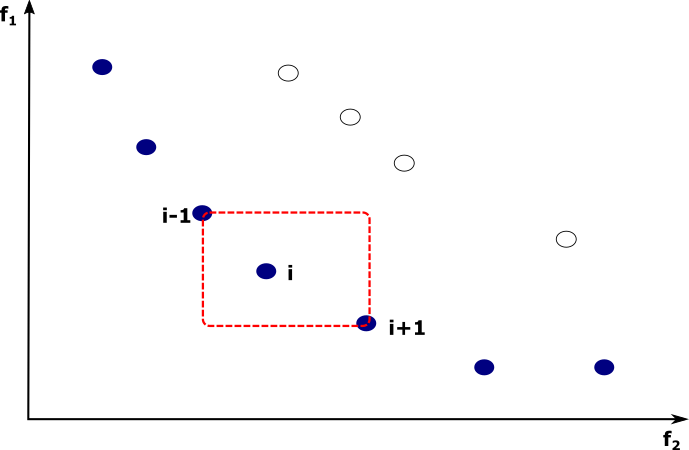
\includegraphics[width=8cm]{CrowdedDistanceSorting}
    \caption{Crowding Distance Sorting in NSGA-II}
    \label{fig:crowdeddistance_sorting}
\end{figure}

\begin{align}
    distance(i) = distance(i) + \frac{f_k(i+1) - f_k(i-1)}{f_k^{max} - f_k^{min}} \qquad \forall \ f_k \in F \label{eq:3.4a} 
\end{align}

More diversity is obtained using solutions with a high crowding distance. \textit{Histogram-based} diversity preserving approaches partition the search space into several hyper-grids defining the neighborhood. The density around a solution is estimated by the number of solutions in the same box of gird \parencite{Talbi2009Metaheuristics:Implementation}. The technique used to measure the distance between solutions is essential for diversity preservation. Diversity in the decision space may be essential to improve the search for some problems. However, some only require diversity in the objective space.

\section{Comparative Analysis of Select Algorithms}
In this chapter, we have extensively discussed different algorithmic approaches that are commonly used to solving combinatorial optimization problems. We have presented algorithms that are typically suited for multiple objective optimization problem section. Through our analysis, we can conclude that using traditional techniques such as local search, tabu search, e.t.c will be more difficult to implement for our \gls{moop}. This is because such techniques yield a single local optimum. A single objective optimizer needs to be run multiple times, using such techniques. Also, good distribution (uniform diversity) is not guaranteed. Thus, a considerable amount of adaptation will be required to use them for our problem domain. In contrast, modern algorithms such as the evolutionary algorithm, Ant Colony Optimization and Bee Colony algorithms are best suited for multiple objective problems, because they can return the Pareto optimal set in a single run. Also, they can be easily decomposed to find the optimal solution for single objectives. Hence, they do not require extra effort than necessary, to be implemented for our problem domain. 

It is impossible to implement all algorithms considered suitable for our problem domain during the duration of this thesis. Thus, we shall be comparing Evolutionary algorithms and Ant Colony optimization. These two choices are based on their popularity for solving Orienteering problems, multi-Objective Knapsack problems and multi-objective problems in general. 

\begin{table}[htpb]
  \caption[Algorithm Comparison]{Selected Algorithm Comparison.}\label{tab:comparison_alg}
  \centering
  \begin{tabular}{l l l l}
    \toprule
       &Evolutionary Algorithm &Ant-Colony \\
    \midrule
      Computational time & \checkmark &  \\
      Applicability to problem domain & \checkmark & \\
      Approximate Pareto front & \checkmark & \checkmark \\
      Diversity Preserving & \checkmark & \checkmark \\
      Applicability to large-sized objectives & & \checkmark \\
      Easier to Implement & \checkmark & \\
    \bottomrule
  \end{tabular}
\end{table}

In table \ref{tab:comparison_alg}, \glspl{ea} and \glspl{aoc} are compared against each other using some desired algorithmic properties we have previously listed in section \ref{sec:alg_approaches} of this chapter. The capabilities of widely used \gls{ea} variants like \gls{nsga}-II, \gls{nsga}-III,\gls{spea}2 were also taken into account. These scores are based on evaluation results gotten from \parencite{Lust2012TheApproach, Florios2010SolvingAlgorithms, Alaya2007AntProblems}. They were chosen because multi-objective knapsack problems were used for evaluation in their studies. A checkmark is awarded, when the algorithm has an advantage over the other for that specific criteria. For example, in comparison to \glspl{aoc}, \glspl{ea} have shown faster computational time in solving multi-objective Knapsack problems. However, there is no known better algorithm between both algorithms for approximating to the Pareto front. \Gls{aoc} as an algorithm is specifically designed to solve path search problems. A graph representation of the knapsack model has to be constructed. This increase the implementation complexity of the \gls{aoc}. Unlike \gls{aoc}, a number of \gls{ea} variants can be directly used for our optimization problem, even without adaptation.

We can conclude that an evolutionary algorithm will be the best-fit algorithmic approach for our \gls{moop}.



 



 